\chapter{Avaliação}
\label{c_avaliacao}
Este capítulo apresenta o contexto de realização da pesquisa e os procedimentos metodológicos adotados. Esta pesquisa tem abordagem qualitativa exploratória, buscando gerar dados descritivos e explanatórios, em vez de demonstrar estatisticamente relações de causa e efeito. O objetivo é compreender e descrever as interações das crianças com a interface de realidade aumentada projetiva durante a programação e depuração de algoritmos. Para isso, a \autoref{sec:contexto} descreve o contexto de realização da pesquisa e a \autoref{sec:participantes} descreve os participantes. Por fim, a \autoref{sec:protocolo} apresenta os experimentos realizados, detalhando a estratégia de coleta de dados e o método de análise destes dados.

\section{Contexto}
\label{sec:contexto}
\subsection{Município}
A coleta de dados ocorreu em um \ac{CDI} no município de Gaspar, no estado de Santa Catarina. A respeito da cidade, O IBGE (Instituto Brasileiro de Geografia e Estatística) estima a população em 70.793 pessoas, com uma densidade demográfica de 150 pessoas por km\textsuperscript{2}. Aproximadamente 40\% da população tem ocupação, sendo que o salário médio dos trabalhadores formais é 2,4 salários-mínimos. O índice de desenvolvimento humano é 0,765, e está acima da média nacional de \. A taxa de mortalidade infantil é 4,42 a cada 1000 nascidos vivos, contra \ no Brasil. A taxa de escolarização entre 6 e 14 anos é de 97,3\%.
\subsection{Centro de Desenvolvimento Infantil}
\label{sec:cdi}
A pesquisa ocorreu em um  \ac{CDI} de um bairro urbano de Gaspar, distante aproximadamente cinco quilômetros do centro da cidade. O local foi selecionado por conveniência, pois o pesquisador conhece uma professora que leciona no local, o que possibilitou a execução de pesquisas em anos anteriores. A pesquisa atual, entretanto, não ocorreu nas turmas desta professora. Além disso, nenhum dos participantes conhecia o brinquedo RoPE. Outro critério para a seleção do centro foi a presença de internet, pois projetor disponível utiliza conexão sem fio local.

O \ac{PPP} do \ac{CDI} apresenta dados históricos e da estrutura física do local. O mesmo foi fundado em 1990, sendo uma parceria entre a prefeitura municipal e a associação de moradores do bairro. Atualmente possui 38 colaboradores, que promovem o atendimento de 246 crianças. A idade atendida vai de zero e cinco anos e onze meses, e há 12 turmas organizadas em três grupos etários: Infância I (0 a 2 anos), Infância II (2 a 4 anos) e Infância III (4 a 6 anos). Dentro de cada grupo etário as turmas também são divididas. Na Infância III, por exemplo, há as turmas de 4 a 5 e de 5 a 6 anos. O espaço tem 9 salas onde as professoras realizam suas atividades, uma biblioteca com aproximadamente 300 livros infantis, um parquinho, banheiros, sala de coordenação e sala do zelador. Além das salas existentes, está em curso a construção de novos espaços no local onde antes havia o parquinho, o qual foi deslocado para um espaço ao lado do CDI. 

O \ac{PPP} do \ac{CDI} apresenta um diagnóstico da comunidade, construído a partir de um questionário. O trabalho apresenta gráficos de pizza, que serão analisados visualmente pois não apresentam dados numericamente (\autoref{fig:contexto_ppp}). Aproximadamente 2/3 das crianças mora com pai e mãe, metade vai de carro ao \ac{CDI}, e quase a metade não tem computador em casa. A respeito dos pais, a maior parte auxilia os filhos nas atividades do \ac{CDI} mas não tem disponibilidade em horário comercial. A renda de aproximadamente a metade das famílias é de 1 a 2 salários-mínimos, e de outra metade vai de 2 a 4.

\begin{figure}[!htbp]
    \centering
    \begin{subfigure}{.3\linewidth}
        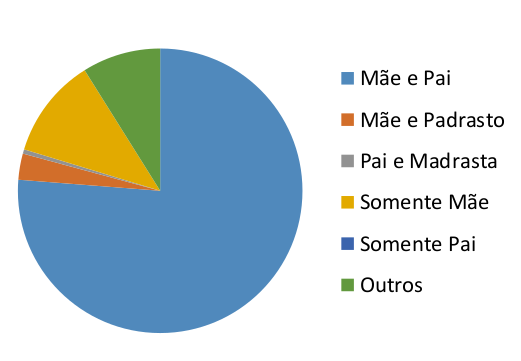
\includegraphics[width=.9\linewidth,fbox]{figs/cdi/mora_com.png}
        \caption{Com quem a criança mora.}
        \label{fig:mora_com}
    \end{subfigure}%
    \begin{subfigure}{.3\textwidth}
        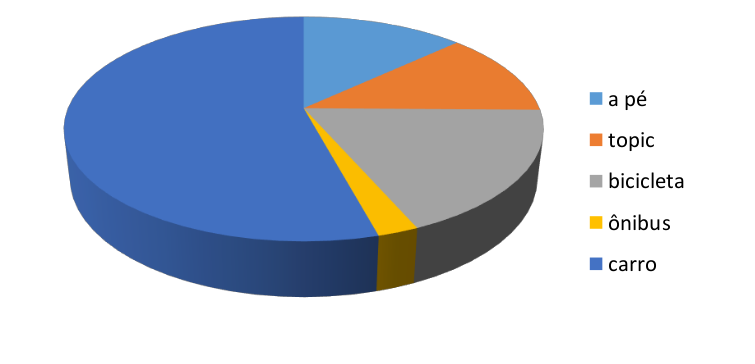
\includegraphics[width=.9\linewidth,fbox]{figs/cdi/meio_transporte.png}
        \caption{Meio de transporte.}
        \label{fig:transporte}
    \end{subfigure}%
   \begin{subfigure}{.3\textwidth}
        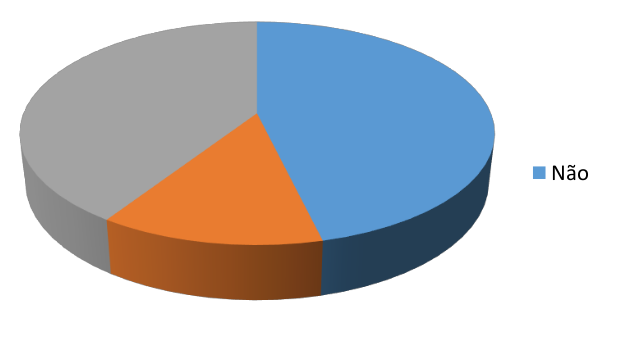
\includegraphics[width=.9\linewidth,fbox]{figs/cdi/tem_computador.png}
        \caption{Tem computador em casa?}
        \label{fig:tem_computador}
    \end{subfigure}
    \begin{subfigure}{.3\textwidth}
        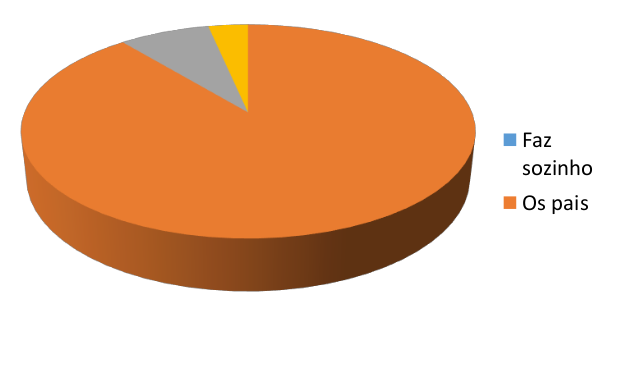
\includegraphics[width=.9\linewidth,fbox]{figs/cdi/pai_auxilia_crianca_atividades.png}
        \caption{Auxílio dos pais nas atividades do CDI}
        \label{fig:pai_auxilia_crianca_atividades}
    \end{subfigure}%
    \begin{subfigure}{.3\textwidth}
        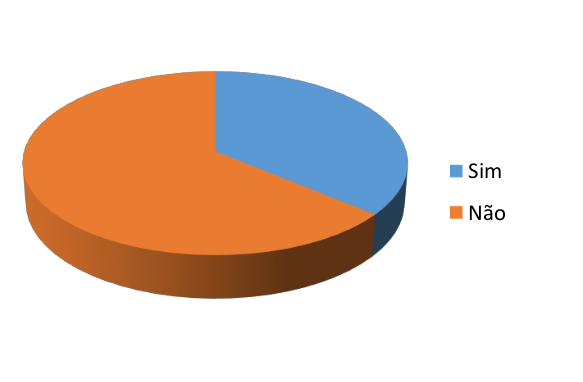
\includegraphics[width=.9\linewidth,fbox]{figs/cdi/disponibilidade_pais_horario_comercial.png}
        \caption{Disponibilidade dos pais em horário comercial.}
        \label{fig:disponibilidade_pais_horario_comercial}
    \end{subfigure}%
     \begin{subfigure}{.3\textwidth}
        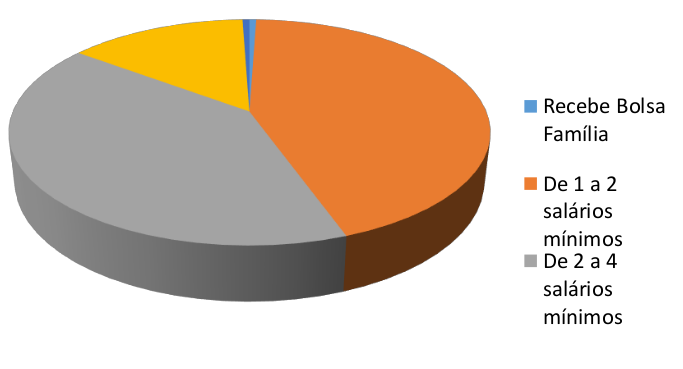
\includegraphics[width=.9\linewidth,fbox]{figs/cdi/renda.png}
        \caption{Renda mensal familiar.}
        \label{fig:renda}
    \end{subfigure}%
    \caption{Dados do Projeto Político Pedagógico do CDI.}
    \label{fig:contexto_ppp}
\end{figure}
Considerando os dados do IBGE e do PPP, infere-se que as condições de vida na região não são precárias, porém a necessidade de trabalho impede o acompanhamento dos filhos em horário comercial. Em horário compatível, porém, os pais buscam auxiliar os filhos nas atividades.

\subsection{Proposta Pedagógica para a Educação Infantil}
Mesmo com as suas particularidades locais, todos os CDIs de Gaspar buscam seguir uma mesma proposta pedagógica alinhada com a rede de ensino do municipal. O documento orientador é a Proposta Pedagógica da Rede Municipal para a Educação Infantil \cite{gaspar_proposta_2010}. Essa proposta foi publicada em 2010, após ser construída coletivamente pelos professores e professoras da Rede Municipal de Educação Infantil. O resultado é um documento que busca nortear o trabalho pedagógico “para e com” as crianças pequenas.

Este “norte” tem duas bases principais: os eixos de Linguagens, Interações e Brincadeiras, e a abordagem metodológica de projetos. Quanto aos eixos, o eixo de Linguagens tem como objetivo incrementar as aprendizagens infantis por meio de atividades que envolvam uso do corpo (linguagem motora); exploração dos sons (linguagem musical); exploração de cores, formas e texturas (linguagem plástica); fala e códigos (linguagem oral e escrita) e noções de espaço, quantidade e números (linguagem matemática). O eixo de Interações diz respeito ao planejamento e organização de situações de contato entre criança-criança, criança-adulto e criança-objeto. Por fim, o eixo das brincadeiras busca aumentar o repertório de interações lúdicas entre as crianças, orientando o educador a observar, coordenar ou integrar-se nas brincadeiras.

Já a Metodologia de Projetos, segundo a proposta, é uma abordagem que permite combinar as intenções pedagógicas do adulto e também estimular a curiosidade da criança. Esse estímulo se dá ao propor projetos em que há investigação de algum tema ou construção de algo com foco em assuntos do mundo infantil (ver \autoref{fig:tres_porquinhos}). Os temas dos projetos surgem em diálogos durante rodas de conversa, passeios ou brincadeiras. Partindo do interesse das crianças, os projetos seguem uma estrutura com hipóteses, perguntas de pesquisa, descrições e comparações. Não há prazo de início e fim, e também não há necessidade de trabalhar diariamente com projetos. Quando nenhum projeto está em curso, trabalha-se seguindo os eixos de Linguagens, Interações e Brincadeiras.

\begin{figure}[!h]
    \centering
    \begin{subfigure}{.45\linewidth}
        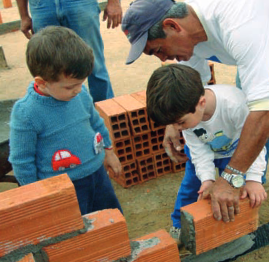
\includegraphics[width=.8\linewidth,fbox]{figs/tres_porquinhos.png}
        \caption{Projeto de construção de casa de tijolos (História dos Três Porquinhos).}
        \source{Proposta Pedagógica da Rede Municipal de Educação Infantil de Gaspar (2010). }
        \label{fig:tres_porquinhos}
    \end{subfigure}%
    \hspace{.05\textwidth}%
    \begin{subfigure}{.45\textwidth}
        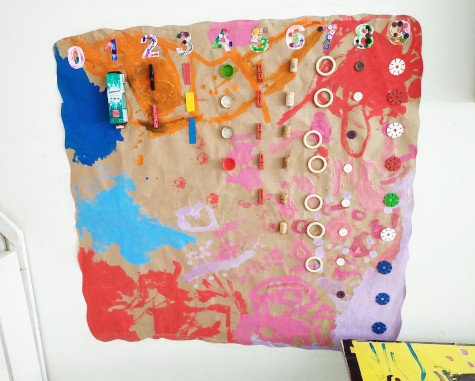
\includegraphics[width=.8\linewidth,fbox]{figs/projeto_numeros_menor.jpeg}
        \caption{Projeto para assimilação de quantidades. Turma de 4 a 5 anos.}
        \source{O autor.}
        \label{fig:projeto_numeros}
    \end{subfigure}%
\end{figure}
A proposta não menciona diretamente o tema das tecnologias digitais. Palavras como \textit{celular} e \textit{computador} não são citadas. Ainda assim, a relação com o “mundo digital” é aderente aos eixos e abordagens metodológicas propostas. As Interações, por exemplo, podem ser favorecidas pelo RoPE AR, quando a criança aperta botões e encaixa blocos que provocam reações em um objeto. Há também o uso de uma Linguagem para comunicar uma sequência de ações à um objeto (o brinquedo RoPE). Por fim, a atividade em si é uma Brincadeira, que segundo a proposta deve envolver elementos acolhedores, desafiadores e inclusivos \cite[p.50]{gaspar_proposta_2010}. 

% restaurante, canto caverna, castelo das bonecas, área de animais aquáticos, robô

\section{Participantes da pesquisa}
\label{sec:participantes}
Apresentado o contexto do local da pesquisa e a proposta pedagógica adotada, é preciso comentar sobre os participantes. A etapa de coleta de dados ocorreu durante quatro dias em um CDI público de um bairro de Gaspar, no estado de Santa Catarina. Participaram 26 crianças com idades entre 4 e 6 anos. Entretanto, a análise considera apenas três dias de visita e a participação de 20 crianças, devido ao descarte de vídeos inadequados\footnote{O posicionamento da câmera impediu ver as ações das crianças ou mais de três crianças interagiram simultâneamente com o brinquedo, sem que o pesquisador conseguisse estruturar a a atividade.}. As crianças e professores participantes estiveram distribuídos em três salas. A primeira sala atende crianças entre 5 e 6 anos, e as outras duas salas (A e B) atendem crianças entre 4 a 5 anos. Cada sala recebe crianças diferentes no período matutino e vespertino.

No primeiro dia a atividade ocorreu na sala de 5 a 6 anos, no período vespertino. No segundo dia a visita ocorreu na segunda sala durante o período vespertino, com crianças de 4 a 5 anos. Por fim, no quarto dia a terceira sala visitada foi a da segunda turma de 4 a 5 anos, tanto de manhã quanto à tarde. Ao fim, quatro grupos de crianças participaram (\autoref{quadro:participants}).

 \begin{quadro}[!h]
 		\setlength{\extrarowheight}{3pt}
        \begin{center}
        \caption{Encontros e participantes}
        \label{quadro:participants}
        \begin{tabular}{@{}llcccc@{}}
            \toprule
            Grupo & Encontro & Turma  & Meninas & Meninos & Professoras \\ \midrule
            1         & Dia 1                       & 5 a 6 anos - Tarde      & 3 & 2 & Daiana e Maria \\
            2         & Dia 2                       & 4 a 5 anos A - Tarde   & 0 & 3 & Paula e Joana \\
            3         & Dia 3                       & 4 a 5 anos B - Manhã & 4 & 2 & Vera e Lúcia \\
            4         & Dia 3                       & 4 a 5 anos B - Tarde   & 2 & 4 & Vera e Lúcia \\ \midrule
            4 grupos          & 3 dias        & 5 turmas     & 9 & 11 & Seis professoras \\ \bottomrule 
            \end{tabular}
        \end{center}
        \sourceauthor
    \end{quadro}

Além das crianças, as professoras de cada uma das três salas também participaram da pesquisa. Cada sala possui uma professora e uma assistente, que serão tratadas aqui como professoras. Todas são mulheres, e possuem de 4 a 28 anos de experiência de trabalho com crianças. Das seis professoras participantes, três responderam diretamente a entrevistas e outras três colaboraram em algum momento por meio de comentários a respeito do projeto ou auxiliando na comunicação com as crianças. As nomes utilizados no texto são fictícios, a fim de evitar a identificação dos participantes.

\section{Ambiente}
As atividades ocorreram em três salas comumente frequentadas pelas crianças. Em todas as salas o projetor ficou em um suporte, posicionado ao lado de uma fonte de energia e afastado de janelas e portas. As luzes das salas foram apagadas, mas isso não modificou o ambiente a ponto de torná-lo escuro (ver \autoref{fig:setting}). No chão à frente do projetor, foram fixadas duas cartolinas brancas para receber as imagens projetadas.

\begin{figure}[!h]
    \centering
    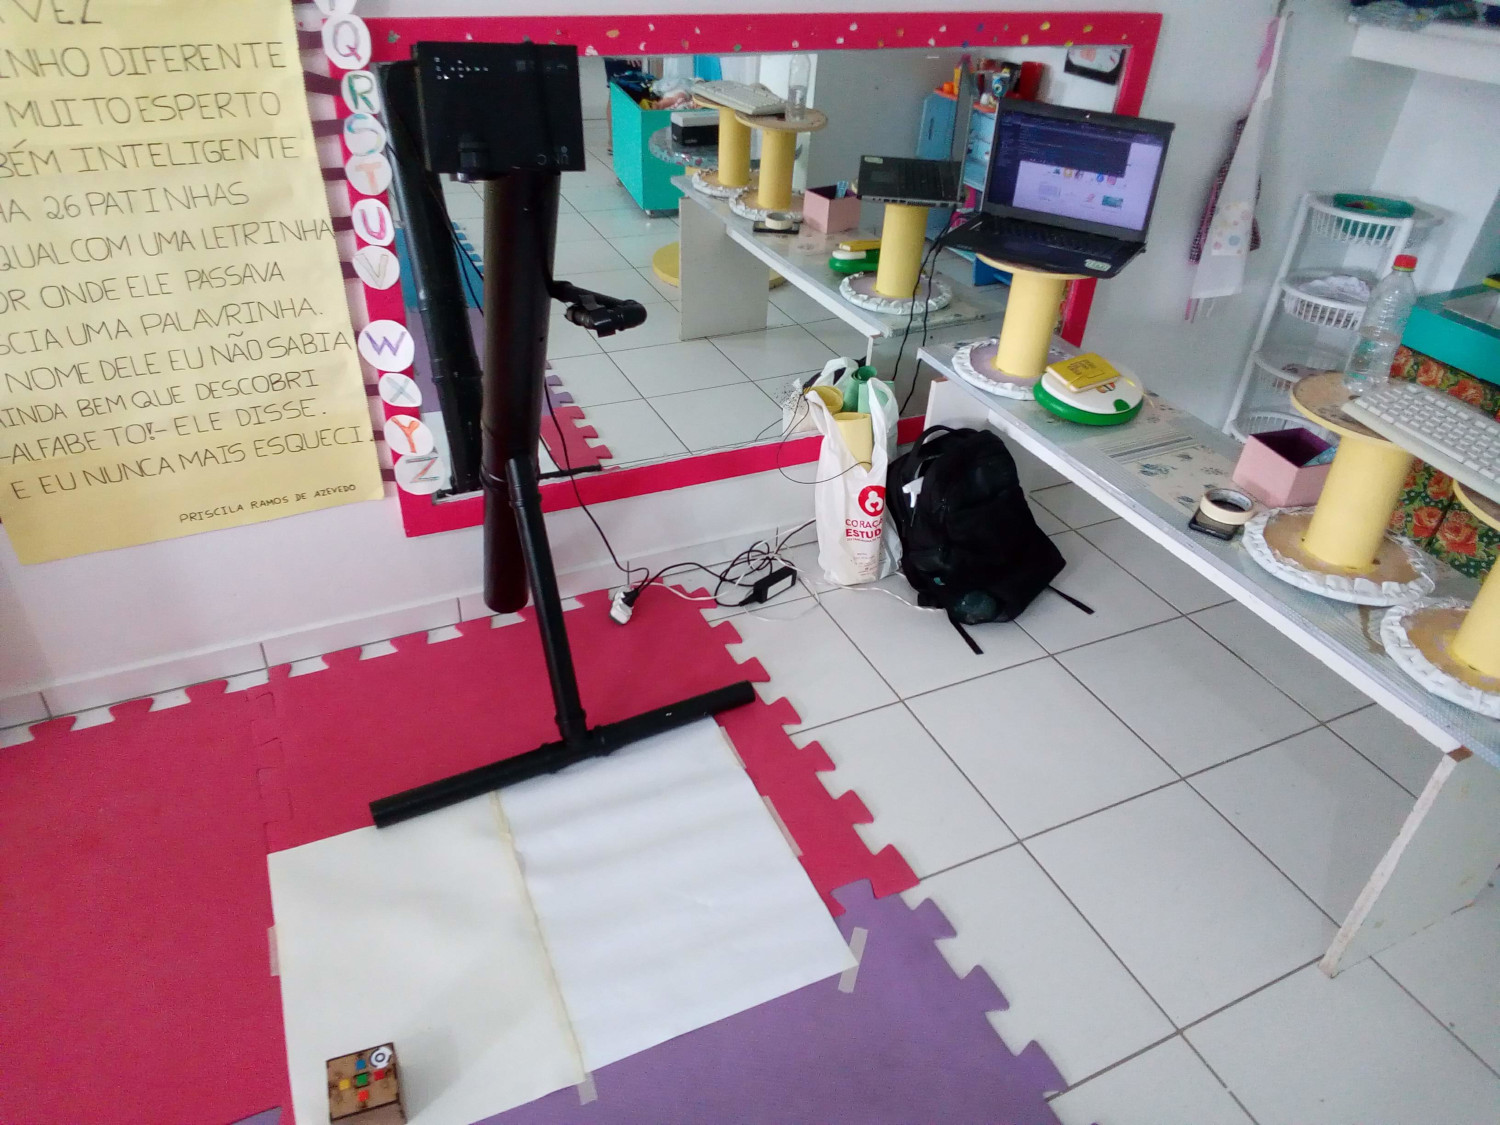
\includegraphics[width=0.8\textwidth,fbox]{figs/setting_projector.jpg}
    \caption{Posicionamento do projetor.}
    \label{fig:setting}
\end{figure}

Durante a organização dos equipamentos, as crianças continuaram suas atividades junto às professoras, porém era perceptível a curiosidade a respeito dos materiais e da figura do pesquisador. Na sala da turma 4-5A há um espaço externo gramado, separado da sala em si. Neste ambiente a professora continuou as atividades no espaço externo, e a programação do RoPE ocorreu dentro da sala com outra professora. As outras duas salas tem espaços amplos, e todas as crianças permaneceram no recinto durante a atividade.

O CDI tem rede de internet sem fio, porém a qualidade do sinal é variável em cada sala. Especificamente na sala 4-5A há dificuldade de manter a conexão. Esse problema foi mencionado pelas professoras e percebido por este pesquisador. As demais salas, porém, tem conexão estável.

\label{sec:protocolo}
Conversa inicial

Apresentação do RoPE

Leitura de código
\begin{itemize}
\item 
\item O que você vê neste desenho? O que está desenhado aqui?
\item Porque você acha que o RoPE está se movendo deste jeito?
\item Como você encaixaria esses desenhos?
\end{itemize}

Tipos de erros



\citeonline{rogers_design_2013} enfatizam a necessidade de envolver o usuário no processo de design, pois são as metas do usuário que direcionam o desenvolvimento de produtos interativos. Esse desenvolvimento deve seguir três princípios. O primeiro é entender quem são os usuários e suas tarefas. No caso desta pesquisa, os usuários são crianças entre \idadeinicial e \idadefinal anos, e as tarefas são solucionar problemas programando o brinquedo RoPE. 

O segundo princípio defendido por \citeonline{rogers_design_2013} são as medições empíricas. Isso indica que durante o desenvolvimento, as reações e o desempenho dos usuários durante a interação com protótipos deve ser observado, medido e analisado. 

O último princípio é o design iterativo. Quando testes apontam problemas, estes devem ser consertados e seguidos de mais testes e observações, num ciclo de projetar-testar-medir-reprojetar. 

A força motriz do design iterativo são as metas do usuário, que são ações que o usuário deseja poder fazer \cite{rogers_design_2013}. Neste trabalho, o alcance das metas de usabilidade se dá quando a criança:

\begin{itemize}
    \item posiciona o brinquedo na posição inicial;
    \item percebe que os blocos representam ações do robô;
    \item sequencia blocos formando um algoritmo;
    \item inicia execução do algoritmo;
    \item altera sequência de blocos; e
    \item percebe blocos destacados durante execução.
\end{itemize}

%Portanto, o protótipo descrito na \autoref{s_prototipo}, será testado iterativamente. Durante os testes, deve-se utilizar documentação por vídeos e diário de bordo. Problemas de usabilidade que impeçam o prosseguimento da atividade  solucionados, e verificados na próxima iteração. As iterações terminam quando as metas de usabilidade forem alcançadas.

Para direcionar a observação, as categorias de análise serão (i) 
para quais elementos da interface as crianças olham;
(ii) se e como as crianças manipulam os blocos; (iii) perguntas realizadas; (iv) se e como as crianças comparam os blocos com os símbolos do robô; (v) como ocorre o início da execução; (vi) em que local e direção posicionam o robô; e (vii) se e como os elementos virtuais são percebidos pelas crianças.

\subsection{Colaboração e Depuração}

A colaboração será observada quando duas ou mais crianças brincarem em conjunto com os blocos. Esse tipo de evento já foi observado em estudos anteriores \cite{sapounidis_tangible_2019, raabe_estudo_2019}, mas precisa ser confirmado neste estudo para afirmar que a interface apresentada tem os benefícios das interfaces tangíveis. 

A depuração será contabilizada de forma simples, e a única condição é haver um ponto específico para o brinquedo chegar. Se o brinquedo se desviar do trajeto, a depuração será contabilizada quando a criança observar, na sequência de blocos, quais comandos provocaram o erro. Essa observação será registrada qualitativamente, por meio de falas e posterior análise de conteúdo \cite{bardin_alise_1979}.

\subsection{Localização e Direção}
A hipótese H2 afirma que a interface promoverá menos erros ligados à localização e direção, quando comparada à programação por botões. Seguindo a classificação de \citeonline{cannon_system_2007}, localização e direção é uma categoria de noções espaciais, entre as quais estão conceitos de posições relativas a um eixo horizontal. Esses conceitos são descritos por palavras como "esquerda", "direita", "frente", "trás" e "lados". 

Para verificar a influência da interface na expressão de direções, a criança deverá programar o RoPE de diferentes perspectivas. Três diferentes perspectivas são possíveis: criança na mesma orientação do brinquedo (visão posterior); criança tendo visão lateral do brinquedo; e a criança tendo visão frontal do brinquedo.

Em cada uma desses três perspectivas, a criança pode programar movimentos lineares ou giratórios. O movimento linear significa ir para frente ou para trás, e o movimento giratório significa girar para esquerda ou direita sobre o próprio eixo. Não se considera diferença entre frente ou trás e esquerda ou direita.

A \autoref{fig:lateralidade} demonstra a sequência de atividades planejada para que a criança programe esses dois tipos de movimento nas três perspectivas. Dada a posição e orientação inicial do RoPE, a bandeira quadriculada indica o ponto de chegada. Em cada uma das atividades, a criança permanece na mesma posição e programa usando blocos de papelão.

\begin{figure}[!hbt]
    \centering
    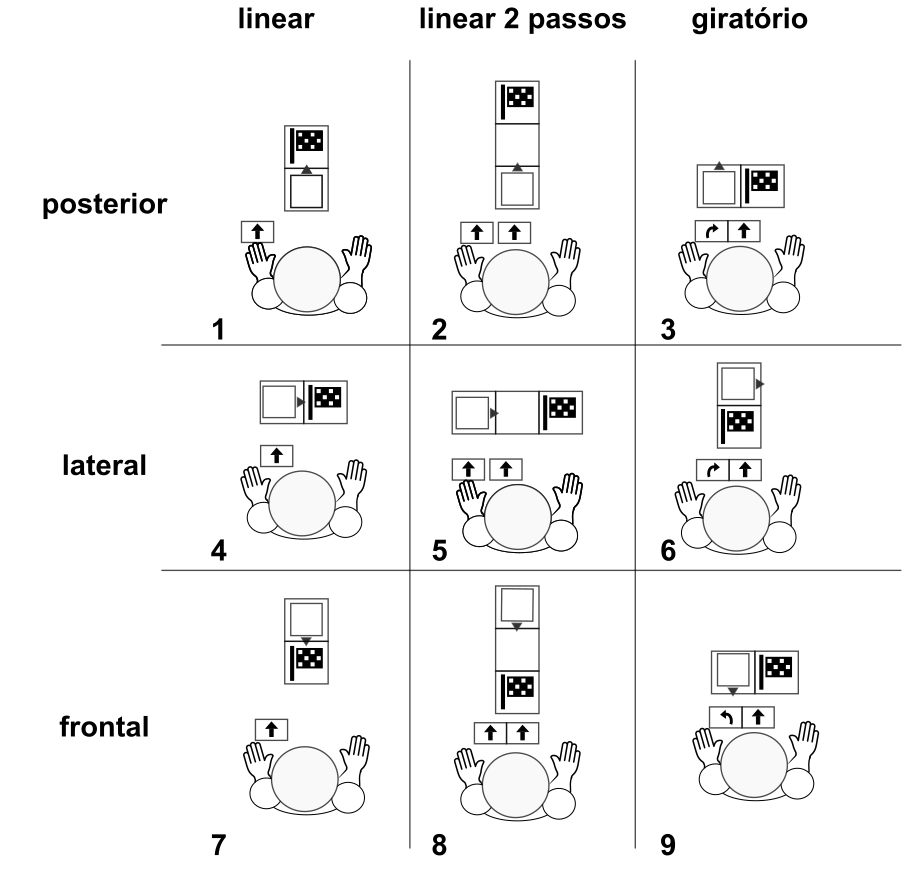
\includegraphics[width=.9\textwidth,fbox]{figs/lateralidade.png}
    \caption{Tarefas para testar lateralidade.}
    \sourceauthor
    \label{fig:lateralidade}
\end{figure}

A variável independente será o tipo de interface de programação (botões, blocos com realidade aumentada) e as variáveis dependentes serão o número de erros e o tempo para finalizar cada atividade.  

A contagem de erros considera as execuções onde os comandos não correspondem exatamente aos necessários para completar a tarefa. Se o brinquedo sair da rota, um adulto deverá recolocá-lo no ponto inicial. O mesmo ocorre se o brinquedo ultrapassar o ponto de chegada.

A contagem de tempo da primeira tarefa inicia com o clique no botão "Iniciar" do aplicativo, e as demais tarefas iniciam quando a tarefa anterior termina. Um tempo limite de 5 minutos por tarefa padroniza o quanto cada criança poderá tentar resolvê-la. Se o tempo limite for alcançado, então as próximas tarefas não serão executadas.

A ordem de aplicação das variáveis independentes será aleatória, ou seja, a criança pode iniciar com a interface de botões ou com os blocos. Isso evita o viés do aprendizado, em que a segunda interface teria resultados melhores pela criança resolver a tarefa com a interface anterior.

